\batchmode
\documentclass[twoside]{book}

% Packages required by doxygen
\usepackage{fixltx2e}
\usepackage{calc}
\usepackage{doxygen}
\usepackage[export]{adjustbox} % also loads graphicx
\usepackage{graphicx}
\usepackage[utf8]{inputenc}
\usepackage{makeidx}
\usepackage{multicol}
\usepackage{multirow}
\PassOptionsToPackage{warn}{textcomp}
\usepackage{textcomp}
\usepackage[nointegrals]{wasysym}
\usepackage[table]{xcolor}

% Font selection
\usepackage[T1]{fontenc}
\usepackage[scaled=.90]{helvet}
\usepackage{courier}
\usepackage{amssymb}
\usepackage{sectsty}
\renewcommand{\familydefault}{\sfdefault}
\allsectionsfont{%
  \fontseries{bc}\selectfont%
  \color{darkgray}%
}
\renewcommand{\DoxyLabelFont}{%
  \fontseries{bc}\selectfont%
  \color{darkgray}%
}
\newcommand{\+}{\discretionary{\mbox{\scriptsize$\hookleftarrow$}}{}{}}

% Page & text layout
\usepackage{geometry}
\geometry{%
  a4paper,%
  top=2.5cm,%
  bottom=2.5cm,%
  left=2.5cm,%
  right=2.5cm%
}
\tolerance=750
\hfuzz=15pt
\hbadness=750
\setlength{\emergencystretch}{15pt}
\setlength{\parindent}{0cm}
\setlength{\parskip}{3ex plus 2ex minus 2ex}
\makeatletter
\renewcommand{\paragraph}{%
  \@startsection{paragraph}{4}{0ex}{-1.0ex}{1.0ex}{%
    \normalfont\normalsize\bfseries\SS@parafont%
  }%
}
\renewcommand{\subparagraph}{%
  \@startsection{subparagraph}{5}{0ex}{-1.0ex}{1.0ex}{%
    \normalfont\normalsize\bfseries\SS@subparafont%
  }%
}
\makeatother

% Headers & footers
\usepackage{fancyhdr}
\pagestyle{fancyplain}
\fancyhead[LE]{\fancyplain{}{\bfseries\thepage}}
\fancyhead[CE]{\fancyplain{}{}}
\fancyhead[RE]{\fancyplain{}{\bfseries\leftmark}}
\fancyhead[LO]{\fancyplain{}{\bfseries\rightmark}}
\fancyhead[CO]{\fancyplain{}{}}
\fancyhead[RO]{\fancyplain{}{\bfseries\thepage}}
\fancyfoot[LE]{\fancyplain{}{}}
\fancyfoot[CE]{\fancyplain{}{}}
\fancyfoot[RE]{\fancyplain{}{\bfseries\scriptsize Generated by Doxygen }}
\fancyfoot[LO]{\fancyplain{}{\bfseries\scriptsize Generated by Doxygen }}
\fancyfoot[CO]{\fancyplain{}{}}
\fancyfoot[RO]{\fancyplain{}{}}
\renewcommand{\footrulewidth}{0.4pt}
\renewcommand{\chaptermark}[1]{%
  \markboth{#1}{}%
}
\renewcommand{\sectionmark}[1]{%
  \markright{\thesection\ #1}%
}

% Indices & bibliography
\usepackage{natbib}
\usepackage[titles]{tocloft}
\setcounter{tocdepth}{3}
\setcounter{secnumdepth}{5}
\makeindex

% Hyperlinks (required, but should be loaded last)
\usepackage{ifpdf}
\ifpdf
  \usepackage[pdftex,pagebackref=true]{hyperref}
\else
  \usepackage[ps2pdf,pagebackref=true]{hyperref}
\fi
\hypersetup{%
  colorlinks=true,%
  linkcolor=blue,%
  citecolor=blue,%
  unicode%
}

% Custom commands
\newcommand{\clearemptydoublepage}{%
  \newpage{\pagestyle{empty}\cleardoublepage}%
}

\usepackage{caption}
\captionsetup{labelsep=space,justification=centering,font={bf},singlelinecheck=off,skip=4pt,position=top}

%===== C O N T E N T S =====

\begin{document}

% Titlepage & ToC
\hypersetup{pageanchor=false,
             bookmarksnumbered=true,
             pdfencoding=unicode
            }
\pagenumbering{alph}
\pagenumbering{arabic}
\hypersetup{pageanchor=true}

%--- Begin generated contents ---
\chapter{Example problem\+: Solution of the 2D unsteady heat equation with restarts}
\label{index}\hypertarget{index}{}\hypertarget{index_q}{}\section{A few quick questions...}\label{index_q}
Since {\ttfamily oomph-\/lib} is developed as open-\/source software, any evidence that the code is being downloaded and used is very helpful for us as it helps to justify our continued work on this project.

We would therefore be extremely grateful if you could provide the information requested in the form below. Pressing the \char`\"{}submit\char`\"{} button will get you to the actual download page.

{\bfseries Note\+:} 
\begin{DoxyItemize}
\item All information will be treated as confidential. 
\item If you provide your email address and check the appropriate box we will add you to our mailing list to inform you of upgrades and bug fixes to the code. Rest assured that the mailing list is {\bfseries very low volume} -- we have better things to do than to bombard you with email. 
\item If you still feel reluctant to provide any of the information requested, feel free to enter some dummy input. The form will check that {\bfseries some} information has been entered but entering your name as \char`\"{}\+Joe Cool\char`\"{} is perfectly acceptable -- this is to discourage people from not providing the information simply because they are too lazy to type... 
\end{DoxyItemize}



 







 

 \hypertarget{index_pdf}{}\section{P\+D\+F file}\label{index_pdf}
A \href{../latex/refman.pdf}{\tt pdf version} of this document is available. \end{document}

\chapter{Namespace Index}
\section{Namespace List}
Here is a list of all namespaces with brief descriptions\+:\begin{DoxyCompactList}
\item\contentsline{section}{\hyperlink{namespaceGlobal__Physical__Variables}{Global\+\_\+\+Physical\+\_\+\+Variables} \\*Global variables that represent physical properties }{\pageref{namespaceGlobal__Physical__Variables}}{}
\item\contentsline{section}{\hyperlink{namespaceoomph}{oomph} }{\pageref{namespaceoomph}}{}
\item\contentsline{section}{\hyperlink{namespacePhysical__Variables}{Physical\+\_\+\+Variables} \\*Namespace for the solution of 2D linear shell equation }{\pageref{namespacePhysical__Variables}}{}
\end{DoxyCompactList}

\chapter{Hierarchical Index}
\section{Class Hierarchy}
This inheritance list is sorted roughly, but not completely, alphabetically\+:\begin{DoxyCompactList}
\item Problem\begin{DoxyCompactList}
\item \contentsline{section}{Unstructured\+Solid\+Problem$<$ E\+L\+E\+M\+E\+NT $>$}{\pageref{classUnstructuredSolidProblem}}{}
\end{DoxyCompactList}
\end{DoxyCompactList}

\chapter{Class Index}
\section{Class List}
Here are the classes, structs, unions and interfaces with brief descriptions\+:\begin{DoxyCompactList}
\item\contentsline{section}{\hyperlink{classPMLProblem}{P\+M\+L\+Problem$<$ E\+L\+E\+M\+E\+N\+T $>$} }{\pageref{classPMLProblem}}{}
\item\contentsline{section}{\hyperlink{classGlobalParameters_1_1TestPMLMapping}{Global\+Parameters\+::\+Test\+P\+M\+L\+Mapping} }{\pageref{classGlobalParameters_1_1TestPMLMapping}}{}
\end{DoxyCompactList}

\chapter{File Index}
\section{File List}
Here is a list of all files with brief descriptions\+:\begin{DoxyCompactList}
\item\contentsline{section}{\hyperlink{jeffery__orbit_8cc}{jeffery\+\_\+orbit.\+cc} }{\pageref{jeffery__orbit_8cc}}{}
\item\contentsline{section}{\hyperlink{jeffery__orbit_8txt__doxygenified_8h}{jeffery\+\_\+orbit.\+txt\+\_\+doxygenified.\+h} }{\pageref{jeffery__orbit_8txt__doxygenified_8h}}{}
\item\contentsline{section}{\hyperlink{my__taylor__hood__elements_8h}{my\+\_\+taylor\+\_\+hood\+\_\+elements.\+h} }{\pageref{my__taylor__hood__elements_8h}}{}
\end{DoxyCompactList}

\chapter{Namespace Documentation}
\hypertarget{namespaceExactSolnForUnsteadyHeat}{}\section{Exact\+Soln\+For\+Unsteady\+Heat Namespace Reference}
\label{namespaceExactSolnForUnsteadyHeat}\index{Exact\+Soln\+For\+Unsteady\+Heat@{Exact\+Soln\+For\+Unsteady\+Heat}}


Namespace for forced exact solution for Unsteady\+Heat equation.  


\subsection*{Functions}
\begin{DoxyCompactItemize}
\item 
void \hyperlink{namespaceExactSolnForUnsteadyHeat_a1d5b22857bd2a7825397daf1cf9c89eb}{get\+\_\+exact\+\_\+u} (const double \&time, const Vector$<$ double $>$ \&x, Vector$<$ double $>$ \&u)
\begin{DoxyCompactList}\small\item\em Exact solution as a Vector. \end{DoxyCompactList}\item 
void \hyperlink{namespaceExactSolnForUnsteadyHeat_a36e38a9c0c7c0bf8916e2d86ac75b4e2}{get\+\_\+exact\+\_\+u} (const double \&time, const Vector$<$ double $>$ \&x, double \&u)
\begin{DoxyCompactList}\small\item\em Exact solution as a scalar. \end{DoxyCompactList}\item 
void \hyperlink{namespaceExactSolnForUnsteadyHeat_ab4e853d6368b1fcdbd6205079687455a}{get\+\_\+source} (const double \&time, const Vector$<$ double $>$ \&x, double \&source)
\begin{DoxyCompactList}\small\item\em Source function to make it an exact solution. \end{DoxyCompactList}\end{DoxyCompactItemize}
\subsection*{Variables}
\begin{DoxyCompactItemize}
\item 
double \hyperlink{namespaceExactSolnForUnsteadyHeat_a188d3472da738e31efb23740c027754c}{Gamma} =10.\+0
\begin{DoxyCompactList}\small\item\em Factor controlling the rate of change. \end{DoxyCompactList}\item 
double \hyperlink{namespaceExactSolnForUnsteadyHeat_a20d04bcf14546becd4bcdf45446be756}{K} =3.\+0
\begin{DoxyCompactList}\small\item\em Wavenumber. \end{DoxyCompactList}\item 
double \hyperlink{namespaceExactSolnForUnsteadyHeat_a630f9e8d892cfcc41cdaef25bfc87ca1}{Phi} =1.\+0
\begin{DoxyCompactList}\small\item\em Angle of bump. \end{DoxyCompactList}\end{DoxyCompactItemize}


\subsection{Detailed Description}
Namespace for forced exact solution for Unsteady\+Heat equation. 

\subsection{Function Documentation}
\mbox{\Hypertarget{namespaceExactSolnForUnsteadyHeat_a1d5b22857bd2a7825397daf1cf9c89eb}\label{namespaceExactSolnForUnsteadyHeat_a1d5b22857bd2a7825397daf1cf9c89eb}} 
\index{Exact\+Soln\+For\+Unsteady\+Heat@{Exact\+Soln\+For\+Unsteady\+Heat}!get\+\_\+exact\+\_\+u@{get\+\_\+exact\+\_\+u}}
\index{get\+\_\+exact\+\_\+u@{get\+\_\+exact\+\_\+u}!Exact\+Soln\+For\+Unsteady\+Heat@{Exact\+Soln\+For\+Unsteady\+Heat}}
\subsubsection{\texorpdfstring{get\+\_\+exact\+\_\+u()}{get\_exact\_u()}\hspace{0.1cm}{\footnotesize\ttfamily [1/2]}}
{\footnotesize\ttfamily void Exact\+Soln\+For\+Unsteady\+Heat\+::get\+\_\+exact\+\_\+u (\begin{DoxyParamCaption}\item[{const double \&}]{time,  }\item[{const Vector$<$ double $>$ \&}]{x,  }\item[{Vector$<$ double $>$ \&}]{u }\end{DoxyParamCaption})}



Exact solution as a Vector. 



Definition at line 69 of file two\+\_\+d\+\_\+unsteady\+\_\+heat\+\_\+t\+\_\+adapt.\+cc.



Referenced by Unsteady\+Heat\+Problem$<$ E\+L\+E\+M\+E\+N\+T $>$\+::actions\+\_\+before\+\_\+implicit\+\_\+timestep(), Unsteady\+Heat\+Problem$<$ E\+L\+E\+M\+E\+N\+T $>$\+::doc\+\_\+solution(), and Unsteady\+Heat\+Problem$<$ E\+L\+E\+M\+E\+N\+T $>$\+::set\+\_\+initial\+\_\+condition().

\mbox{\Hypertarget{namespaceExactSolnForUnsteadyHeat_a36e38a9c0c7c0bf8916e2d86ac75b4e2}\label{namespaceExactSolnForUnsteadyHeat_a36e38a9c0c7c0bf8916e2d86ac75b4e2}} 
\index{Exact\+Soln\+For\+Unsteady\+Heat@{Exact\+Soln\+For\+Unsteady\+Heat}!get\+\_\+exact\+\_\+u@{get\+\_\+exact\+\_\+u}}
\index{get\+\_\+exact\+\_\+u@{get\+\_\+exact\+\_\+u}!Exact\+Soln\+For\+Unsteady\+Heat@{Exact\+Soln\+For\+Unsteady\+Heat}}
\subsubsection{\texorpdfstring{get\+\_\+exact\+\_\+u()}{get\_exact\_u()}\hspace{0.1cm}{\footnotesize\ttfamily [2/2]}}
{\footnotesize\ttfamily void Exact\+Soln\+For\+Unsteady\+Heat\+::get\+\_\+exact\+\_\+u (\begin{DoxyParamCaption}\item[{const double \&}]{time,  }\item[{const Vector$<$ double $>$ \&}]{x,  }\item[{double \&}]{u }\end{DoxyParamCaption})}



Exact solution as a scalar. 



Definition at line 78 of file two\+\_\+d\+\_\+unsteady\+\_\+heat\+\_\+t\+\_\+adapt.\+cc.

\mbox{\Hypertarget{namespaceExactSolnForUnsteadyHeat_ab4e853d6368b1fcdbd6205079687455a}\label{namespaceExactSolnForUnsteadyHeat_ab4e853d6368b1fcdbd6205079687455a}} 
\index{Exact\+Soln\+For\+Unsteady\+Heat@{Exact\+Soln\+For\+Unsteady\+Heat}!get\+\_\+source@{get\+\_\+source}}
\index{get\+\_\+source@{get\+\_\+source}!Exact\+Soln\+For\+Unsteady\+Heat@{Exact\+Soln\+For\+Unsteady\+Heat}}
\subsubsection{\texorpdfstring{get\+\_\+source()}{get\_source()}}
{\footnotesize\ttfamily void Exact\+Soln\+For\+Unsteady\+Heat\+::get\+\_\+source (\begin{DoxyParamCaption}\item[{const double \&}]{time,  }\item[{const Vector$<$ double $>$ \&}]{x,  }\item[{double \&}]{source }\end{DoxyParamCaption})}



Source function to make it an exact solution. 



Definition at line 86 of file two\+\_\+d\+\_\+unsteady\+\_\+heat\+\_\+t\+\_\+adapt.\+cc.



Referenced by main().



\subsection{Variable Documentation}
\mbox{\Hypertarget{namespaceExactSolnForUnsteadyHeat_a188d3472da738e31efb23740c027754c}\label{namespaceExactSolnForUnsteadyHeat_a188d3472da738e31efb23740c027754c}} 
\index{Exact\+Soln\+For\+Unsteady\+Heat@{Exact\+Soln\+For\+Unsteady\+Heat}!Gamma@{Gamma}}
\index{Gamma@{Gamma}!Exact\+Soln\+For\+Unsteady\+Heat@{Exact\+Soln\+For\+Unsteady\+Heat}}
\subsubsection{\texorpdfstring{Gamma}{Gamma}}
{\footnotesize\ttfamily double Exact\+Soln\+For\+Unsteady\+Heat\+::\+Gamma =10.\+0}



Factor controlling the rate of change. 



Definition at line 60 of file two\+\_\+d\+\_\+unsteady\+\_\+heat\+\_\+t\+\_\+adapt.\+cc.



Referenced by Unsteady\+Heat\+Problem$<$ E\+L\+E\+M\+E\+N\+T $>$\+::\+Unsteady\+Heat\+Problem().

\mbox{\Hypertarget{namespaceExactSolnForUnsteadyHeat_a20d04bcf14546becd4bcdf45446be756}\label{namespaceExactSolnForUnsteadyHeat_a20d04bcf14546becd4bcdf45446be756}} 
\index{Exact\+Soln\+For\+Unsteady\+Heat@{Exact\+Soln\+For\+Unsteady\+Heat}!K@{K}}
\index{K@{K}!Exact\+Soln\+For\+Unsteady\+Heat@{Exact\+Soln\+For\+Unsteady\+Heat}}
\subsubsection{\texorpdfstring{K}{K}}
{\footnotesize\ttfamily double Exact\+Soln\+For\+Unsteady\+Heat\+::K =3.\+0}



Wavenumber. 



Definition at line 63 of file two\+\_\+d\+\_\+unsteady\+\_\+heat\+\_\+t\+\_\+adapt.\+cc.



Referenced by Unsteady\+Heat\+Problem$<$ E\+L\+E\+M\+E\+N\+T $>$\+::\+Unsteady\+Heat\+Problem().

\mbox{\Hypertarget{namespaceExactSolnForUnsteadyHeat_a630f9e8d892cfcc41cdaef25bfc87ca1}\label{namespaceExactSolnForUnsteadyHeat_a630f9e8d892cfcc41cdaef25bfc87ca1}} 
\index{Exact\+Soln\+For\+Unsteady\+Heat@{Exact\+Soln\+For\+Unsteady\+Heat}!Phi@{Phi}}
\index{Phi@{Phi}!Exact\+Soln\+For\+Unsteady\+Heat@{Exact\+Soln\+For\+Unsteady\+Heat}}
\subsubsection{\texorpdfstring{Phi}{Phi}}
{\footnotesize\ttfamily double Exact\+Soln\+For\+Unsteady\+Heat\+::\+Phi =1.\+0}



Angle of bump. 



Definition at line 66 of file two\+\_\+d\+\_\+unsteady\+\_\+heat\+\_\+t\+\_\+adapt.\+cc.


\chapter{Class Documentation}
\hypertarget{classUnsteadyHeatProblem}{}\section{Unsteady\+Heat\+Problem$<$ E\+L\+E\+M\+E\+NT $>$ Class Template Reference}
\label{classUnsteadyHeatProblem}\index{Unsteady\+Heat\+Problem$<$ E\+L\+E\+M\+E\+N\+T $>$@{Unsteady\+Heat\+Problem$<$ E\+L\+E\+M\+E\+N\+T $>$}}


Unsteady\+Heat problem.  


Inheritance diagram for Unsteady\+Heat\+Problem$<$ E\+L\+E\+M\+E\+NT $>$\+:\begin{figure}[H]
\begin{center}
\leavevmode
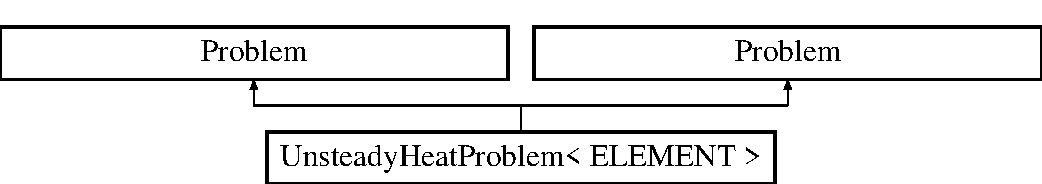
\includegraphics[height=2.000000cm]{classUnsteadyHeatProblem}
\end{center}
\end{figure}
\subsection*{Public Member Functions}
\begin{DoxyCompactItemize}
\item 
\hyperlink{classUnsteadyHeatProblem_abd3a46eea132b1e5872be6a6309a51b2}{Unsteady\+Heat\+Problem} (Unsteady\+Heat\+Equations$<$ 2 $>$\+::Unsteady\+Heat\+Source\+Fct\+Pt source\+\_\+fct\+\_\+pt)
\begin{DoxyCompactList}\small\item\em Constructor. \end{DoxyCompactList}\item 
\hyperlink{classUnsteadyHeatProblem_acd342b40828d9e18b3571e00b3d34add}{$\sim$\+Unsteady\+Heat\+Problem} ()
\begin{DoxyCompactList}\small\item\em Destructor (empty) \end{DoxyCompactList}\item 
void \hyperlink{classUnsteadyHeatProblem_a88e3d534b5904f7c10ce6a8fbd6df0ea}{actions\+\_\+after\+\_\+newton\+\_\+solve} ()
\begin{DoxyCompactList}\small\item\em Update the problem specs after solve (empty) \end{DoxyCompactList}\item 
void \hyperlink{classUnsteadyHeatProblem_aa1ee8fbe2a5439d1cacb37131e0f81c6}{actions\+\_\+before\+\_\+newton\+\_\+solve} ()
\begin{DoxyCompactList}\small\item\em Update the problem specs before solve (empty) \end{DoxyCompactList}\item 
void \hyperlink{classUnsteadyHeatProblem_afd14cbe343adfa39e3b8b2ca681c5020}{actions\+\_\+after\+\_\+implicit\+\_\+timestep} ()
\begin{DoxyCompactList}\small\item\em Update the problem specs after solve (empty) \end{DoxyCompactList}\item 
void \hyperlink{classUnsteadyHeatProblem_a7074e52f6a3a791549687e1b4ddd059a}{actions\+\_\+before\+\_\+implicit\+\_\+timestep} ()
\begin{DoxyCompactList}\small\item\em Update the problem specs before next timestep\+: Set Dirchlet boundary conditions from exact solution. \end{DoxyCompactList}\item 
void \hyperlink{classUnsteadyHeatProblem_a98de3ed2d9cf5409323121bbb482bc1b}{set\+\_\+initial\+\_\+condition} ()
\begin{DoxyCompactList}\small\item\em Set initial condition (incl previous timesteps) according to specified function. \end{DoxyCompactList}\item 
void \hyperlink{classUnsteadyHeatProblem_a2c0c4b762d2dbde7396dca2a6750f433}{doc\+\_\+solution} (Doc\+Info \&doc\+\_\+info, ofstream \&trace\+\_\+file)
\begin{DoxyCompactList}\small\item\em Doc the solution. \end{DoxyCompactList}\item 
\hyperlink{classUnsteadyHeatProblem_abd3a46eea132b1e5872be6a6309a51b2}{Unsteady\+Heat\+Problem} (Unsteady\+Heat\+Equations$<$ 2 $>$\+::Unsteady\+Heat\+Source\+Fct\+Pt source\+\_\+fct\+\_\+pt)
\begin{DoxyCompactList}\small\item\em Constructor. \end{DoxyCompactList}\item 
\hyperlink{classUnsteadyHeatProblem_acd342b40828d9e18b3571e00b3d34add}{$\sim$\+Unsteady\+Heat\+Problem} ()
\begin{DoxyCompactList}\small\item\em Destructor (empty) \end{DoxyCompactList}\item 
void \hyperlink{classUnsteadyHeatProblem_a88e3d534b5904f7c10ce6a8fbd6df0ea}{actions\+\_\+after\+\_\+newton\+\_\+solve} ()
\begin{DoxyCompactList}\small\item\em Update the problem specs after solve (empty) \end{DoxyCompactList}\item 
void \hyperlink{classUnsteadyHeatProblem_aa1ee8fbe2a5439d1cacb37131e0f81c6}{actions\+\_\+before\+\_\+newton\+\_\+solve} ()
\begin{DoxyCompactList}\small\item\em Update the problem specs before solve (empty) \end{DoxyCompactList}\item 
void \hyperlink{classUnsteadyHeatProblem_afd14cbe343adfa39e3b8b2ca681c5020}{actions\+\_\+after\+\_\+implicit\+\_\+timestep} ()
\begin{DoxyCompactList}\small\item\em Update the problem specs after solve (empty) \end{DoxyCompactList}\item 
void \hyperlink{classUnsteadyHeatProblem_a7074e52f6a3a791549687e1b4ddd059a}{actions\+\_\+before\+\_\+implicit\+\_\+timestep} ()
\begin{DoxyCompactList}\small\item\em Update the problem specs before next timestep\+: Set Dirchlet boundary conditions from exact solution. \end{DoxyCompactList}\item 
void \hyperlink{classUnsteadyHeatProblem_a98de3ed2d9cf5409323121bbb482bc1b}{set\+\_\+initial\+\_\+condition} ()
\begin{DoxyCompactList}\small\item\em Set initial condition (incl previous timesteps) according to specified function. \end{DoxyCompactList}\item 
void \hyperlink{classUnsteadyHeatProblem_a2c0c4b762d2dbde7396dca2a6750f433}{doc\+\_\+solution} (Doc\+Info \&doc\+\_\+info, ofstream \&trace\+\_\+file)
\begin{DoxyCompactList}\small\item\em Doc the solution. \end{DoxyCompactList}\item 
void \hyperlink{classUnsteadyHeatProblem_a9a60874a6471414819301705f1a2afd1}{dump\+\_\+it} (ofstream \&dump\+\_\+file)
\begin{DoxyCompactList}\small\item\em Dump problem to disk to allow for restart. \end{DoxyCompactList}\item 
void \hyperlink{classUnsteadyHeatProblem_ad0a4a1c1da24f6d62f64b0d40be31709}{restart} (ifstream \&restart\+\_\+file)
\begin{DoxyCompactList}\small\item\em Read problem for restart from specified restart file. \end{DoxyCompactList}\end{DoxyCompactItemize}
\subsection*{Private Attributes}
\begin{DoxyCompactItemize}
\item 
Unsteady\+Heat\+Equations$<$ 2 $>$\+::Unsteady\+Heat\+Source\+Fct\+Pt \hyperlink{classUnsteadyHeatProblem_a923d1a0bd45b1cd747a5b4558ae3f190}{Source\+\_\+fct\+\_\+pt}
\begin{DoxyCompactList}\small\item\em Pointer to source function. \end{DoxyCompactList}\item 
Node $\ast$ \hyperlink{classUnsteadyHeatProblem_ac0cf04bd0b915f02b171fd50cae13874}{Control\+\_\+node\+\_\+pt}
\begin{DoxyCompactList}\small\item\em Pointer to control node at which the solution is documented. \end{DoxyCompactList}\end{DoxyCompactItemize}


\subsection{Detailed Description}
\subsubsection*{template$<$class E\+L\+E\+M\+E\+NT$>$\newline
class Unsteady\+Heat\+Problem$<$ E\+L\+E\+M\+E\+N\+T $>$}

Unsteady\+Heat problem. 

Definition at line 95 of file two\+\_\+d\+\_\+unsteady\+\_\+heat.\+cc.



\subsection{Constructor \& Destructor Documentation}
\mbox{\Hypertarget{classUnsteadyHeatProblem_abd3a46eea132b1e5872be6a6309a51b2}\label{classUnsteadyHeatProblem_abd3a46eea132b1e5872be6a6309a51b2}} 
\index{Unsteady\+Heat\+Problem@{Unsteady\+Heat\+Problem}!Unsteady\+Heat\+Problem@{Unsteady\+Heat\+Problem}}
\index{Unsteady\+Heat\+Problem@{Unsteady\+Heat\+Problem}!Unsteady\+Heat\+Problem@{Unsteady\+Heat\+Problem}}
\subsubsection{\texorpdfstring{Unsteady\+Heat\+Problem()}{UnsteadyHeatProblem()}\hspace{0.1cm}{\footnotesize\ttfamily [1/2]}}
{\footnotesize\ttfamily template$<$class E\+L\+E\+M\+E\+NT $>$ \\
\hyperlink{classUnsteadyHeatProblem}{Unsteady\+Heat\+Problem}$<$ E\+L\+E\+M\+E\+NT $>$\+::\hyperlink{classUnsteadyHeatProblem}{Unsteady\+Heat\+Problem} (\begin{DoxyParamCaption}\item[{Unsteady\+Heat\+Equations$<$ 2 $>$\+::Unsteady\+Heat\+Source\+Fct\+Pt}]{source\+\_\+fct\+\_\+pt }\end{DoxyParamCaption})}



Constructor. 

Constructor for Unsteady\+Heat problem in square domain. 

Definition at line 142 of file two\+\_\+d\+\_\+unsteady\+\_\+heat.\+cc.



References Unsteady\+Heat\+Problem$<$ E\+L\+E\+M\+E\+N\+T $>$\+::\+Control\+\_\+node\+\_\+pt, Exact\+Soln\+For\+Unsteady\+Heat\+::K, and Unsteady\+Heat\+Problem$<$ E\+L\+E\+M\+E\+N\+T $>$\+::\+Source\+\_\+fct\+\_\+pt.



Referenced by Unsteady\+Heat\+Problem$<$ E\+L\+E\+M\+E\+N\+T $>$\+::actions\+\_\+after\+\_\+implicit\+\_\+timestep().

\mbox{\Hypertarget{classUnsteadyHeatProblem_acd342b40828d9e18b3571e00b3d34add}\label{classUnsteadyHeatProblem_acd342b40828d9e18b3571e00b3d34add}} 
\index{Unsteady\+Heat\+Problem@{Unsteady\+Heat\+Problem}!````~Unsteady\+Heat\+Problem@{$\sim$\+Unsteady\+Heat\+Problem}}
\index{````~Unsteady\+Heat\+Problem@{$\sim$\+Unsteady\+Heat\+Problem}!Unsteady\+Heat\+Problem@{Unsteady\+Heat\+Problem}}
\subsubsection{\texorpdfstring{$\sim$\+Unsteady\+Heat\+Problem()}{~UnsteadyHeatProblem()}\hspace{0.1cm}{\footnotesize\ttfamily [1/2]}}
{\footnotesize\ttfamily template$<$class E\+L\+E\+M\+E\+NT$>$ \\
\hyperlink{classUnsteadyHeatProblem}{Unsteady\+Heat\+Problem}$<$ E\+L\+E\+M\+E\+NT $>$\+::$\sim$\hyperlink{classUnsteadyHeatProblem}{Unsteady\+Heat\+Problem} (\begin{DoxyParamCaption}{ }\end{DoxyParamCaption})\hspace{0.3cm}{\ttfamily [inline]}}



Destructor (empty) 



Definition at line 105 of file two\+\_\+d\+\_\+unsteady\+\_\+heat.\+cc.

\mbox{\Hypertarget{classUnsteadyHeatProblem_abd3a46eea132b1e5872be6a6309a51b2}\label{classUnsteadyHeatProblem_abd3a46eea132b1e5872be6a6309a51b2}} 
\index{Unsteady\+Heat\+Problem@{Unsteady\+Heat\+Problem}!Unsteady\+Heat\+Problem@{Unsteady\+Heat\+Problem}}
\index{Unsteady\+Heat\+Problem@{Unsteady\+Heat\+Problem}!Unsteady\+Heat\+Problem@{Unsteady\+Heat\+Problem}}
\subsubsection{\texorpdfstring{Unsteady\+Heat\+Problem()}{UnsteadyHeatProblem()}\hspace{0.1cm}{\footnotesize\ttfamily [2/2]}}
{\footnotesize\ttfamily template$<$class E\+L\+E\+M\+E\+NT$>$ \\
\hyperlink{classUnsteadyHeatProblem}{Unsteady\+Heat\+Problem}$<$ E\+L\+E\+M\+E\+NT $>$\+::\hyperlink{classUnsteadyHeatProblem}{Unsteady\+Heat\+Problem} (\begin{DoxyParamCaption}\item[{Unsteady\+Heat\+Equations$<$ 2 $>$\+::Unsteady\+Heat\+Source\+Fct\+Pt}]{source\+\_\+fct\+\_\+pt }\end{DoxyParamCaption})}



Constructor. 

\mbox{\Hypertarget{classUnsteadyHeatProblem_acd342b40828d9e18b3571e00b3d34add}\label{classUnsteadyHeatProblem_acd342b40828d9e18b3571e00b3d34add}} 
\index{Unsteady\+Heat\+Problem@{Unsteady\+Heat\+Problem}!````~Unsteady\+Heat\+Problem@{$\sim$\+Unsteady\+Heat\+Problem}}
\index{````~Unsteady\+Heat\+Problem@{$\sim$\+Unsteady\+Heat\+Problem}!Unsteady\+Heat\+Problem@{Unsteady\+Heat\+Problem}}
\subsubsection{\texorpdfstring{$\sim$\+Unsteady\+Heat\+Problem()}{~UnsteadyHeatProblem()}\hspace{0.1cm}{\footnotesize\ttfamily [2/2]}}
{\footnotesize\ttfamily template$<$class E\+L\+E\+M\+E\+NT$>$ \\
\hyperlink{classUnsteadyHeatProblem}{Unsteady\+Heat\+Problem}$<$ E\+L\+E\+M\+E\+NT $>$\+::$\sim$\hyperlink{classUnsteadyHeatProblem}{Unsteady\+Heat\+Problem} (\begin{DoxyParamCaption}{ }\end{DoxyParamCaption})\hspace{0.3cm}{\ttfamily [inline]}}



Destructor (empty) 



Definition at line 105 of file two\+\_\+d\+\_\+unsteady\+\_\+heat\+\_\+restarted.\+cc.



\subsection{Member Function Documentation}
\mbox{\Hypertarget{classUnsteadyHeatProblem_afd14cbe343adfa39e3b8b2ca681c5020}\label{classUnsteadyHeatProblem_afd14cbe343adfa39e3b8b2ca681c5020}} 
\index{Unsteady\+Heat\+Problem@{Unsteady\+Heat\+Problem}!actions\+\_\+after\+\_\+implicit\+\_\+timestep@{actions\+\_\+after\+\_\+implicit\+\_\+timestep}}
\index{actions\+\_\+after\+\_\+implicit\+\_\+timestep@{actions\+\_\+after\+\_\+implicit\+\_\+timestep}!Unsteady\+Heat\+Problem@{Unsteady\+Heat\+Problem}}
\subsubsection{\texorpdfstring{actions\+\_\+after\+\_\+implicit\+\_\+timestep()}{actions\_after\_implicit\_timestep()}\hspace{0.1cm}{\footnotesize\ttfamily [1/2]}}
{\footnotesize\ttfamily template$<$class E\+L\+E\+M\+E\+NT$>$ \\
void \hyperlink{classUnsteadyHeatProblem}{Unsteady\+Heat\+Problem}$<$ E\+L\+E\+M\+E\+NT $>$\+::actions\+\_\+after\+\_\+implicit\+\_\+timestep (\begin{DoxyParamCaption}{ }\end{DoxyParamCaption})\hspace{0.3cm}{\ttfamily [inline]}}



Update the problem specs after solve (empty) 



Definition at line 114 of file two\+\_\+d\+\_\+unsteady\+\_\+heat.\+cc.

\mbox{\Hypertarget{classUnsteadyHeatProblem_afd14cbe343adfa39e3b8b2ca681c5020}\label{classUnsteadyHeatProblem_afd14cbe343adfa39e3b8b2ca681c5020}} 
\index{Unsteady\+Heat\+Problem@{Unsteady\+Heat\+Problem}!actions\+\_\+after\+\_\+implicit\+\_\+timestep@{actions\+\_\+after\+\_\+implicit\+\_\+timestep}}
\index{actions\+\_\+after\+\_\+implicit\+\_\+timestep@{actions\+\_\+after\+\_\+implicit\+\_\+timestep}!Unsteady\+Heat\+Problem@{Unsteady\+Heat\+Problem}}
\subsubsection{\texorpdfstring{actions\+\_\+after\+\_\+implicit\+\_\+timestep()}{actions\_after\_implicit\_timestep()}\hspace{0.1cm}{\footnotesize\ttfamily [2/2]}}
{\footnotesize\ttfamily template$<$class E\+L\+E\+M\+E\+NT$>$ \\
void \hyperlink{classUnsteadyHeatProblem}{Unsteady\+Heat\+Problem}$<$ E\+L\+E\+M\+E\+NT $>$\+::actions\+\_\+after\+\_\+implicit\+\_\+timestep (\begin{DoxyParamCaption}{ }\end{DoxyParamCaption})\hspace{0.3cm}{\ttfamily [inline]}}



Update the problem specs after solve (empty) 



Definition at line 114 of file two\+\_\+d\+\_\+unsteady\+\_\+heat\+\_\+restarted.\+cc.



References Unsteady\+Heat\+Problem$<$ E\+L\+E\+M\+E\+N\+T $>$\+::actions\+\_\+before\+\_\+implicit\+\_\+timestep(), Unsteady\+Heat\+Problem$<$ E\+L\+E\+M\+E\+N\+T $>$\+::doc\+\_\+solution(), Exact\+Soln\+For\+Unsteady\+Heat\+::get\+\_\+exact\+\_\+u(), Exact\+Soln\+For\+Unsteady\+Heat\+::K, Unsteady\+Heat\+Problem$<$ E\+L\+E\+M\+E\+N\+T $>$\+::set\+\_\+initial\+\_\+condition(), and Unsteady\+Heat\+Problem$<$ E\+L\+E\+M\+E\+N\+T $>$\+::\+Unsteady\+Heat\+Problem().

\mbox{\Hypertarget{classUnsteadyHeatProblem_a88e3d534b5904f7c10ce6a8fbd6df0ea}\label{classUnsteadyHeatProblem_a88e3d534b5904f7c10ce6a8fbd6df0ea}} 
\index{Unsteady\+Heat\+Problem@{Unsteady\+Heat\+Problem}!actions\+\_\+after\+\_\+newton\+\_\+solve@{actions\+\_\+after\+\_\+newton\+\_\+solve}}
\index{actions\+\_\+after\+\_\+newton\+\_\+solve@{actions\+\_\+after\+\_\+newton\+\_\+solve}!Unsteady\+Heat\+Problem@{Unsteady\+Heat\+Problem}}
\subsubsection{\texorpdfstring{actions\+\_\+after\+\_\+newton\+\_\+solve()}{actions\_after\_newton\_solve()}\hspace{0.1cm}{\footnotesize\ttfamily [1/2]}}
{\footnotesize\ttfamily template$<$class E\+L\+E\+M\+E\+NT$>$ \\
void \hyperlink{classUnsteadyHeatProblem}{Unsteady\+Heat\+Problem}$<$ E\+L\+E\+M\+E\+NT $>$\+::actions\+\_\+after\+\_\+newton\+\_\+solve (\begin{DoxyParamCaption}{ }\end{DoxyParamCaption})\hspace{0.3cm}{\ttfamily [inline]}}



Update the problem specs after solve (empty) 



Definition at line 108 of file two\+\_\+d\+\_\+unsteady\+\_\+heat.\+cc.

\mbox{\Hypertarget{classUnsteadyHeatProblem_a88e3d534b5904f7c10ce6a8fbd6df0ea}\label{classUnsteadyHeatProblem_a88e3d534b5904f7c10ce6a8fbd6df0ea}} 
\index{Unsteady\+Heat\+Problem@{Unsteady\+Heat\+Problem}!actions\+\_\+after\+\_\+newton\+\_\+solve@{actions\+\_\+after\+\_\+newton\+\_\+solve}}
\index{actions\+\_\+after\+\_\+newton\+\_\+solve@{actions\+\_\+after\+\_\+newton\+\_\+solve}!Unsteady\+Heat\+Problem@{Unsteady\+Heat\+Problem}}
\subsubsection{\texorpdfstring{actions\+\_\+after\+\_\+newton\+\_\+solve()}{actions\_after\_newton\_solve()}\hspace{0.1cm}{\footnotesize\ttfamily [2/2]}}
{\footnotesize\ttfamily template$<$class E\+L\+E\+M\+E\+NT$>$ \\
void \hyperlink{classUnsteadyHeatProblem}{Unsteady\+Heat\+Problem}$<$ E\+L\+E\+M\+E\+NT $>$\+::actions\+\_\+after\+\_\+newton\+\_\+solve (\begin{DoxyParamCaption}{ }\end{DoxyParamCaption})\hspace{0.3cm}{\ttfamily [inline]}}



Update the problem specs after solve (empty) 



Definition at line 108 of file two\+\_\+d\+\_\+unsteady\+\_\+heat\+\_\+restarted.\+cc.

\mbox{\Hypertarget{classUnsteadyHeatProblem_a7074e52f6a3a791549687e1b4ddd059a}\label{classUnsteadyHeatProblem_a7074e52f6a3a791549687e1b4ddd059a}} 
\index{Unsteady\+Heat\+Problem@{Unsteady\+Heat\+Problem}!actions\+\_\+before\+\_\+implicit\+\_\+timestep@{actions\+\_\+before\+\_\+implicit\+\_\+timestep}}
\index{actions\+\_\+before\+\_\+implicit\+\_\+timestep@{actions\+\_\+before\+\_\+implicit\+\_\+timestep}!Unsteady\+Heat\+Problem@{Unsteady\+Heat\+Problem}}
\subsubsection{\texorpdfstring{actions\+\_\+before\+\_\+implicit\+\_\+timestep()}{actions\_before\_implicit\_timestep()}\hspace{0.1cm}{\footnotesize\ttfamily [1/2]}}
{\footnotesize\ttfamily template$<$class E\+L\+E\+M\+E\+NT $>$ \\
void \hyperlink{classUnsteadyHeatProblem}{Unsteady\+Heat\+Problem}$<$ E\+L\+E\+M\+E\+NT $>$\+::actions\+\_\+before\+\_\+implicit\+\_\+timestep (\begin{DoxyParamCaption}{ }\end{DoxyParamCaption})}



Update the problem specs before next timestep\+: Set Dirchlet boundary conditions from exact solution. 

Actions before timestep\+: update the domain, then reset the boundary conditions for the current time. 

Definition at line 232 of file two\+\_\+d\+\_\+unsteady\+\_\+heat.\+cc.



References Exact\+Soln\+For\+Unsteady\+Heat\+::get\+\_\+exact\+\_\+u().



Referenced by Unsteady\+Heat\+Problem$<$ E\+L\+E\+M\+E\+N\+T $>$\+::actions\+\_\+after\+\_\+implicit\+\_\+timestep().

\mbox{\Hypertarget{classUnsteadyHeatProblem_a7074e52f6a3a791549687e1b4ddd059a}\label{classUnsteadyHeatProblem_a7074e52f6a3a791549687e1b4ddd059a}} 
\index{Unsteady\+Heat\+Problem@{Unsteady\+Heat\+Problem}!actions\+\_\+before\+\_\+implicit\+\_\+timestep@{actions\+\_\+before\+\_\+implicit\+\_\+timestep}}
\index{actions\+\_\+before\+\_\+implicit\+\_\+timestep@{actions\+\_\+before\+\_\+implicit\+\_\+timestep}!Unsteady\+Heat\+Problem@{Unsteady\+Heat\+Problem}}
\subsubsection{\texorpdfstring{actions\+\_\+before\+\_\+implicit\+\_\+timestep()}{actions\_before\_implicit\_timestep()}\hspace{0.1cm}{\footnotesize\ttfamily [2/2]}}
{\footnotesize\ttfamily template$<$class E\+L\+E\+M\+E\+NT$>$ \\
void \hyperlink{classUnsteadyHeatProblem}{Unsteady\+Heat\+Problem}$<$ E\+L\+E\+M\+E\+NT $>$\+::actions\+\_\+before\+\_\+implicit\+\_\+timestep (\begin{DoxyParamCaption}{ }\end{DoxyParamCaption})}



Update the problem specs before next timestep\+: Set Dirchlet boundary conditions from exact solution. 

\mbox{\Hypertarget{classUnsteadyHeatProblem_aa1ee8fbe2a5439d1cacb37131e0f81c6}\label{classUnsteadyHeatProblem_aa1ee8fbe2a5439d1cacb37131e0f81c6}} 
\index{Unsteady\+Heat\+Problem@{Unsteady\+Heat\+Problem}!actions\+\_\+before\+\_\+newton\+\_\+solve@{actions\+\_\+before\+\_\+newton\+\_\+solve}}
\index{actions\+\_\+before\+\_\+newton\+\_\+solve@{actions\+\_\+before\+\_\+newton\+\_\+solve}!Unsteady\+Heat\+Problem@{Unsteady\+Heat\+Problem}}
\subsubsection{\texorpdfstring{actions\+\_\+before\+\_\+newton\+\_\+solve()}{actions\_before\_newton\_solve()}\hspace{0.1cm}{\footnotesize\ttfamily [1/2]}}
{\footnotesize\ttfamily template$<$class E\+L\+E\+M\+E\+NT$>$ \\
void \hyperlink{classUnsteadyHeatProblem}{Unsteady\+Heat\+Problem}$<$ E\+L\+E\+M\+E\+NT $>$\+::actions\+\_\+before\+\_\+newton\+\_\+solve (\begin{DoxyParamCaption}{ }\end{DoxyParamCaption})\hspace{0.3cm}{\ttfamily [inline]}}



Update the problem specs before solve (empty) 



Definition at line 111 of file two\+\_\+d\+\_\+unsteady\+\_\+heat\+\_\+restarted.\+cc.

\mbox{\Hypertarget{classUnsteadyHeatProblem_aa1ee8fbe2a5439d1cacb37131e0f81c6}\label{classUnsteadyHeatProblem_aa1ee8fbe2a5439d1cacb37131e0f81c6}} 
\index{Unsteady\+Heat\+Problem@{Unsteady\+Heat\+Problem}!actions\+\_\+before\+\_\+newton\+\_\+solve@{actions\+\_\+before\+\_\+newton\+\_\+solve}}
\index{actions\+\_\+before\+\_\+newton\+\_\+solve@{actions\+\_\+before\+\_\+newton\+\_\+solve}!Unsteady\+Heat\+Problem@{Unsteady\+Heat\+Problem}}
\subsubsection{\texorpdfstring{actions\+\_\+before\+\_\+newton\+\_\+solve()}{actions\_before\_newton\_solve()}\hspace{0.1cm}{\footnotesize\ttfamily [2/2]}}
{\footnotesize\ttfamily template$<$class E\+L\+E\+M\+E\+NT$>$ \\
void \hyperlink{classUnsteadyHeatProblem}{Unsteady\+Heat\+Problem}$<$ E\+L\+E\+M\+E\+NT $>$\+::actions\+\_\+before\+\_\+newton\+\_\+solve (\begin{DoxyParamCaption}{ }\end{DoxyParamCaption})\hspace{0.3cm}{\ttfamily [inline]}}



Update the problem specs before solve (empty) 



Definition at line 111 of file two\+\_\+d\+\_\+unsteady\+\_\+heat.\+cc.

\mbox{\Hypertarget{classUnsteadyHeatProblem_a2c0c4b762d2dbde7396dca2a6750f433}\label{classUnsteadyHeatProblem_a2c0c4b762d2dbde7396dca2a6750f433}} 
\index{Unsteady\+Heat\+Problem@{Unsteady\+Heat\+Problem}!doc\+\_\+solution@{doc\+\_\+solution}}
\index{doc\+\_\+solution@{doc\+\_\+solution}!Unsteady\+Heat\+Problem@{Unsteady\+Heat\+Problem}}
\subsubsection{\texorpdfstring{doc\+\_\+solution()}{doc\_solution()}\hspace{0.1cm}{\footnotesize\ttfamily [1/2]}}
{\footnotesize\ttfamily template$<$class E\+L\+E\+M\+E\+NT$>$ \\
void \hyperlink{classUnsteadyHeatProblem}{Unsteady\+Heat\+Problem}$<$ E\+L\+E\+M\+E\+NT $>$\+::doc\+\_\+solution (\begin{DoxyParamCaption}\item[{Doc\+Info \&}]{doc\+\_\+info,  }\item[{ofstream \&}]{trace\+\_\+file }\end{DoxyParamCaption})}



Doc the solution. 

\mbox{\Hypertarget{classUnsteadyHeatProblem_a2c0c4b762d2dbde7396dca2a6750f433}\label{classUnsteadyHeatProblem_a2c0c4b762d2dbde7396dca2a6750f433}} 
\index{Unsteady\+Heat\+Problem@{Unsteady\+Heat\+Problem}!doc\+\_\+solution@{doc\+\_\+solution}}
\index{doc\+\_\+solution@{doc\+\_\+solution}!Unsteady\+Heat\+Problem@{Unsteady\+Heat\+Problem}}
\subsubsection{\texorpdfstring{doc\+\_\+solution()}{doc\_solution()}\hspace{0.1cm}{\footnotesize\ttfamily [2/2]}}
{\footnotesize\ttfamily template$<$class E\+L\+E\+M\+E\+NT $>$ \\
void \hyperlink{classUnsteadyHeatProblem}{Unsteady\+Heat\+Problem}$<$ E\+L\+E\+M\+E\+NT $>$\+::doc\+\_\+solution (\begin{DoxyParamCaption}\item[{Doc\+Info \&}]{doc\+\_\+info,  }\item[{ofstream \&}]{trace\+\_\+file }\end{DoxyParamCaption})}



Doc the solution. 



Definition at line 331 of file two\+\_\+d\+\_\+unsteady\+\_\+heat.\+cc.



References Unsteady\+Heat\+Problem$<$ E\+L\+E\+M\+E\+N\+T $>$\+::\+Control\+\_\+node\+\_\+pt, and Exact\+Soln\+For\+Unsteady\+Heat\+::get\+\_\+exact\+\_\+u().



Referenced by Unsteady\+Heat\+Problem$<$ E\+L\+E\+M\+E\+N\+T $>$\+::actions\+\_\+after\+\_\+implicit\+\_\+timestep(), main(), and Unsteady\+Heat\+Problem$<$ E\+L\+E\+M\+E\+N\+T $>$\+::set\+\_\+initial\+\_\+condition().

\mbox{\Hypertarget{classUnsteadyHeatProblem_a9a60874a6471414819301705f1a2afd1}\label{classUnsteadyHeatProblem_a9a60874a6471414819301705f1a2afd1}} 
\index{Unsteady\+Heat\+Problem@{Unsteady\+Heat\+Problem}!dump\+\_\+it@{dump\+\_\+it}}
\index{dump\+\_\+it@{dump\+\_\+it}!Unsteady\+Heat\+Problem@{Unsteady\+Heat\+Problem}}
\subsubsection{\texorpdfstring{dump\+\_\+it()}{dump\_it()}}
{\footnotesize\ttfamily template$<$class E\+L\+E\+M\+E\+NT $>$ \\
void \hyperlink{classUnsteadyHeatProblem}{Unsteady\+Heat\+Problem}$<$ E\+L\+E\+M\+E\+NT $>$\+::dump\+\_\+it (\begin{DoxyParamCaption}\item[{ofstream \&}]{dump\+\_\+file }\end{DoxyParamCaption})}



Dump problem to disk to allow for restart. 

Dump the solution to disk to allow for restart. 

Definition at line 500 of file two\+\_\+d\+\_\+unsteady\+\_\+heat\+\_\+restarted.\+cc.

\mbox{\Hypertarget{classUnsteadyHeatProblem_ad0a4a1c1da24f6d62f64b0d40be31709}\label{classUnsteadyHeatProblem_ad0a4a1c1da24f6d62f64b0d40be31709}} 
\index{Unsteady\+Heat\+Problem@{Unsteady\+Heat\+Problem}!restart@{restart}}
\index{restart@{restart}!Unsteady\+Heat\+Problem@{Unsteady\+Heat\+Problem}}
\subsubsection{\texorpdfstring{restart()}{restart()}}
{\footnotesize\ttfamily template$<$class E\+L\+E\+M\+E\+NT $>$ \\
void \hyperlink{classUnsteadyHeatProblem}{Unsteady\+Heat\+Problem}$<$ E\+L\+E\+M\+E\+NT $>$\+::restart (\begin{DoxyParamCaption}\item[{ifstream \&}]{restart\+\_\+file }\end{DoxyParamCaption})}



Read problem for restart from specified restart file. 

Read solution from disk for restart. 

Definition at line 514 of file two\+\_\+d\+\_\+unsteady\+\_\+heat\+\_\+restarted.\+cc.

\mbox{\Hypertarget{classUnsteadyHeatProblem_a98de3ed2d9cf5409323121bbb482bc1b}\label{classUnsteadyHeatProblem_a98de3ed2d9cf5409323121bbb482bc1b}} 
\index{Unsteady\+Heat\+Problem@{Unsteady\+Heat\+Problem}!set\+\_\+initial\+\_\+condition@{set\+\_\+initial\+\_\+condition}}
\index{set\+\_\+initial\+\_\+condition@{set\+\_\+initial\+\_\+condition}!Unsteady\+Heat\+Problem@{Unsteady\+Heat\+Problem}}
\subsubsection{\texorpdfstring{set\+\_\+initial\+\_\+condition()}{set\_initial\_condition()}\hspace{0.1cm}{\footnotesize\ttfamily [1/2]}}
{\footnotesize\ttfamily template$<$class E\+L\+E\+M\+E\+NT$>$ \\
void \hyperlink{classUnsteadyHeatProblem}{Unsteady\+Heat\+Problem}$<$ E\+L\+E\+M\+E\+NT $>$\+::set\+\_\+initial\+\_\+condition (\begin{DoxyParamCaption}{ }\end{DoxyParamCaption})}



Set initial condition (incl previous timesteps) according to specified function. 

\mbox{\Hypertarget{classUnsteadyHeatProblem_a98de3ed2d9cf5409323121bbb482bc1b}\label{classUnsteadyHeatProblem_a98de3ed2d9cf5409323121bbb482bc1b}} 
\index{Unsteady\+Heat\+Problem@{Unsteady\+Heat\+Problem}!set\+\_\+initial\+\_\+condition@{set\+\_\+initial\+\_\+condition}}
\index{set\+\_\+initial\+\_\+condition@{set\+\_\+initial\+\_\+condition}!Unsteady\+Heat\+Problem@{Unsteady\+Heat\+Problem}}
\subsubsection{\texorpdfstring{set\+\_\+initial\+\_\+condition()}{set\_initial\_condition()}\hspace{0.1cm}{\footnotesize\ttfamily [2/2]}}
{\footnotesize\ttfamily template$<$class E\+L\+E\+M\+E\+NT $>$ \\
void \hyperlink{classUnsteadyHeatProblem}{Unsteady\+Heat\+Problem}$<$ E\+L\+E\+M\+E\+NT $>$\+::set\+\_\+initial\+\_\+condition (\begin{DoxyParamCaption}{ }\end{DoxyParamCaption})}



Set initial condition (incl previous timesteps) according to specified function. 

Set initial condition\+: Assign previous and current values from exact solution or from restart file.

Set initial condition\+: Assign previous and current values from exact solution. 

Definition at line 265 of file two\+\_\+d\+\_\+unsteady\+\_\+heat.\+cc.



References Unsteady\+Heat\+Problem$<$ E\+L\+E\+M\+E\+N\+T $>$\+::doc\+\_\+solution(), and Exact\+Soln\+For\+Unsteady\+Heat\+::get\+\_\+exact\+\_\+u().



Referenced by Unsteady\+Heat\+Problem$<$ E\+L\+E\+M\+E\+N\+T $>$\+::actions\+\_\+after\+\_\+implicit\+\_\+timestep(), and main().



\subsection{Member Data Documentation}
\mbox{\Hypertarget{classUnsteadyHeatProblem_ac0cf04bd0b915f02b171fd50cae13874}\label{classUnsteadyHeatProblem_ac0cf04bd0b915f02b171fd50cae13874}} 
\index{Unsteady\+Heat\+Problem@{Unsteady\+Heat\+Problem}!Control\+\_\+node\+\_\+pt@{Control\+\_\+node\+\_\+pt}}
\index{Control\+\_\+node\+\_\+pt@{Control\+\_\+node\+\_\+pt}!Unsteady\+Heat\+Problem@{Unsteady\+Heat\+Problem}}
\subsubsection{\texorpdfstring{Control\+\_\+node\+\_\+pt}{Control\_node\_pt}}
{\footnotesize\ttfamily template$<$class E\+L\+E\+M\+E\+NT$>$ \\
Node $\ast$ \hyperlink{classUnsteadyHeatProblem}{Unsteady\+Heat\+Problem}$<$ E\+L\+E\+M\+E\+NT $>$\+::Control\+\_\+node\+\_\+pt\hspace{0.3cm}{\ttfamily [private]}}



Pointer to control node at which the solution is documented. 



Definition at line 133 of file two\+\_\+d\+\_\+unsteady\+\_\+heat.\+cc.



Referenced by Unsteady\+Heat\+Problem$<$ E\+L\+E\+M\+E\+N\+T $>$\+::doc\+\_\+solution(), and Unsteady\+Heat\+Problem$<$ E\+L\+E\+M\+E\+N\+T $>$\+::\+Unsteady\+Heat\+Problem().

\mbox{\Hypertarget{classUnsteadyHeatProblem_a923d1a0bd45b1cd747a5b4558ae3f190}\label{classUnsteadyHeatProblem_a923d1a0bd45b1cd747a5b4558ae3f190}} 
\index{Unsteady\+Heat\+Problem@{Unsteady\+Heat\+Problem}!Source\+\_\+fct\+\_\+pt@{Source\+\_\+fct\+\_\+pt}}
\index{Source\+\_\+fct\+\_\+pt@{Source\+\_\+fct\+\_\+pt}!Unsteady\+Heat\+Problem@{Unsteady\+Heat\+Problem}}
\subsubsection{\texorpdfstring{Source\+\_\+fct\+\_\+pt}{Source\_fct\_pt}}
{\footnotesize\ttfamily template$<$class E\+L\+E\+M\+E\+NT$>$ \\
Unsteady\+Heat\+Equations$<$ 2 $>$\+::Unsteady\+Heat\+Source\+Fct\+Pt \hyperlink{classUnsteadyHeatProblem}{Unsteady\+Heat\+Problem}$<$ E\+L\+E\+M\+E\+NT $>$\+::Source\+\_\+fct\+\_\+pt\hspace{0.3cm}{\ttfamily [private]}}



Pointer to source function. 



Definition at line 130 of file two\+\_\+d\+\_\+unsteady\+\_\+heat.\+cc.



Referenced by Unsteady\+Heat\+Problem$<$ E\+L\+E\+M\+E\+N\+T $>$\+::\+Unsteady\+Heat\+Problem().



The documentation for this class was generated from the following files\+:\begin{DoxyCompactItemize}
\item 
\hyperlink{two__d__unsteady__heat_8cc}{two\+\_\+d\+\_\+unsteady\+\_\+heat.\+cc}\item 
\hyperlink{two__d__unsteady__heat__restarted_8cc}{two\+\_\+d\+\_\+unsteady\+\_\+heat\+\_\+restarted.\+cc}\end{DoxyCompactItemize}

\chapter{File Documentation}
\hypertarget{two__d__unsteady__heat_8cc}{}\section{two\+\_\+d\+\_\+unsteady\+\_\+heat.\+cc File Reference}
\label{two__d__unsteady__heat_8cc}\index{two\+\_\+d\+\_\+unsteady\+\_\+heat.\+cc@{two\+\_\+d\+\_\+unsteady\+\_\+heat.\+cc}}
\subsection*{Classes}
\begin{DoxyCompactItemize}
\item 
class \hyperlink{classUnsteadyHeatProblem}{Unsteady\+Heat\+Problem$<$ E\+L\+E\+M\+E\+N\+T $>$}
\begin{DoxyCompactList}\small\item\em Unsteady\+Heat problem. \end{DoxyCompactList}\end{DoxyCompactItemize}
\subsection*{Namespaces}
\begin{DoxyCompactItemize}
\item 
 \hyperlink{namespaceExactSolnForUnsteadyHeat}{Exact\+Soln\+For\+Unsteady\+Heat}
\begin{DoxyCompactList}\small\item\em Namespace for unforced exact solution for Unsteady\+Heat equation. \end{DoxyCompactList}\end{DoxyCompactItemize}
\subsection*{Functions}
\begin{DoxyCompactItemize}
\item 
void \hyperlink{namespaceExactSolnForUnsteadyHeat_a1d5b22857bd2a7825397daf1cf9c89eb}{Exact\+Soln\+For\+Unsteady\+Heat\+::get\+\_\+exact\+\_\+u} (const double \&time, const Vector$<$ double $>$ \&x, Vector$<$ double $>$ \&u)
\begin{DoxyCompactList}\small\item\em Exact solution as a Vector. \end{DoxyCompactList}\item 
void \hyperlink{namespaceExactSolnForUnsteadyHeat_a36e38a9c0c7c0bf8916e2d86ac75b4e2}{Exact\+Soln\+For\+Unsteady\+Heat\+::get\+\_\+exact\+\_\+u} (const double \&time, const Vector$<$ double $>$ \&x, double \&u)
\begin{DoxyCompactList}\small\item\em Exact solution as a scalar. \end{DoxyCompactList}\item 
void \hyperlink{namespaceExactSolnForUnsteadyHeat_ab4e853d6368b1fcdbd6205079687455a}{Exact\+Soln\+For\+Unsteady\+Heat\+::get\+\_\+source} (const double \&time, const Vector$<$ double $>$ \&x, double \&source)
\begin{DoxyCompactList}\small\item\em Source function to make it an exact solution. \end{DoxyCompactList}\item 
int \hyperlink{two__d__unsteady__heat_8cc_ae66f6b31b5ad750f1fe042a706a4e3d4}{main} ()
\begin{DoxyCompactList}\small\item\em Driver code for unsteady heat equation. \end{DoxyCompactList}\end{DoxyCompactItemize}
\subsection*{Variables}
\begin{DoxyCompactItemize}
\item 
double \hyperlink{namespaceExactSolnForUnsteadyHeat_a20d04bcf14546becd4bcdf45446be756}{Exact\+Soln\+For\+Unsteady\+Heat\+::K} =10
\begin{DoxyCompactList}\small\item\em Decay factor. \end{DoxyCompactList}\item 
double \hyperlink{namespaceExactSolnForUnsteadyHeat_a630f9e8d892cfcc41cdaef25bfc87ca1}{Exact\+Soln\+For\+Unsteady\+Heat\+::\+Phi} =1.\+0
\begin{DoxyCompactList}\small\item\em Angle of bump. \end{DoxyCompactList}\end{DoxyCompactItemize}


\subsection{Function Documentation}
\mbox{\Hypertarget{two__d__unsteady__heat_8cc_ae66f6b31b5ad750f1fe042a706a4e3d4}\label{two__d__unsteady__heat_8cc_ae66f6b31b5ad750f1fe042a706a4e3d4}} 
\index{two\+\_\+d\+\_\+unsteady\+\_\+heat.\+cc@{two\+\_\+d\+\_\+unsteady\+\_\+heat.\+cc}!main@{main}}
\index{main@{main}!two\+\_\+d\+\_\+unsteady\+\_\+heat.\+cc@{two\+\_\+d\+\_\+unsteady\+\_\+heat.\+cc}}
\subsubsection{\texorpdfstring{main()}{main()}}
{\footnotesize\ttfamily int main (\begin{DoxyParamCaption}{ }\end{DoxyParamCaption})}



Driver code for unsteady heat equation. 



Definition at line 418 of file two\+\_\+d\+\_\+unsteady\+\_\+heat.\+cc.



References Unsteady\+Heat\+Problem$<$ E\+L\+E\+M\+E\+N\+T $>$\+::doc\+\_\+solution(), Exact\+Soln\+For\+Unsteady\+Heat\+::get\+\_\+source(), and Unsteady\+Heat\+Problem$<$ E\+L\+E\+M\+E\+N\+T $>$\+::set\+\_\+initial\+\_\+condition().


\hypertarget{two__d__unsteady__heat2_8txt__doxygenified_8h}{}\section{two\+\_\+d\+\_\+unsteady\+\_\+heat2.\+txt\+\_\+doxygenified.\+h File Reference}
\label{two__d__unsteady__heat2_8txt__doxygenified_8h}\index{two\+\_\+d\+\_\+unsteady\+\_\+heat2.\+txt\+\_\+doxygenified.\+h@{two\+\_\+d\+\_\+unsteady\+\_\+heat2.\+txt\+\_\+doxygenified.\+h}}

\hypertarget{two__d__unsteady__heat__restarted_8cc}{}\section{two\+\_\+d\+\_\+unsteady\+\_\+heat\+\_\+restarted.\+cc File Reference}
\label{two__d__unsteady__heat__restarted_8cc}\index{two\+\_\+d\+\_\+unsteady\+\_\+heat\+\_\+restarted.\+cc@{two\+\_\+d\+\_\+unsteady\+\_\+heat\+\_\+restarted.\+cc}}
\subsection*{Classes}
\begin{DoxyCompactItemize}
\item 
class \hyperlink{classUnsteadyHeatProblem}{Unsteady\+Heat\+Problem$<$ E\+L\+E\+M\+E\+N\+T $>$}
\begin{DoxyCompactList}\small\item\em Unsteady\+Heat problem. \end{DoxyCompactList}\end{DoxyCompactItemize}
\subsection*{Namespaces}
\begin{DoxyCompactItemize}
\item 
 \hyperlink{namespaceExactSolnForUnsteadyHeat}{Exact\+Soln\+For\+Unsteady\+Heat}
\begin{DoxyCompactList}\small\item\em Namespace for unforced exact solution for Unsteady\+Heat equation. \end{DoxyCompactList}\end{DoxyCompactItemize}
\subsection*{Functions}
\begin{DoxyCompactItemize}
\item 
void \hyperlink{namespaceExactSolnForUnsteadyHeat_a1d5b22857bd2a7825397daf1cf9c89eb}{Exact\+Soln\+For\+Unsteady\+Heat\+::get\+\_\+exact\+\_\+u} (const double \&time, const Vector$<$ double $>$ \&x, Vector$<$ double $>$ \&u)
\begin{DoxyCompactList}\small\item\em Exact solution as a Vector. \end{DoxyCompactList}\item 
void \hyperlink{namespaceExactSolnForUnsteadyHeat_a36e38a9c0c7c0bf8916e2d86ac75b4e2}{Exact\+Soln\+For\+Unsteady\+Heat\+::get\+\_\+exact\+\_\+u} (const double \&time, const Vector$<$ double $>$ \&x, double \&u)
\begin{DoxyCompactList}\small\item\em Exact solution as a scalar. \end{DoxyCompactList}\item 
void \hyperlink{namespaceExactSolnForUnsteadyHeat_ab4e853d6368b1fcdbd6205079687455a}{Exact\+Soln\+For\+Unsteady\+Heat\+::get\+\_\+source} (const double \&time, const Vector$<$ double $>$ \&x, double \&source)
\begin{DoxyCompactList}\small\item\em Source function to make it an exact solution. \end{DoxyCompactList}\item 
int \hyperlink{two__d__unsteady__heat__restarted_8cc_a0ddf1224851353fc92bfbff6f499fa97}{main} (int argc, char $\ast$argv\mbox{[}$\,$\mbox{]})
\begin{DoxyCompactList}\small\item\em Driver code for unsteady heat equation with option for restart from disk\+: Only a single command line argument is allowed. If specified it is interpreted as the name of the restart file. \end{DoxyCompactList}\end{DoxyCompactItemize}


\subsection{Function Documentation}
\mbox{\Hypertarget{two__d__unsteady__heat__restarted_8cc_a0ddf1224851353fc92bfbff6f499fa97}\label{two__d__unsteady__heat__restarted_8cc_a0ddf1224851353fc92bfbff6f499fa97}} 
\index{two\+\_\+d\+\_\+unsteady\+\_\+heat\+\_\+restarted.\+cc@{two\+\_\+d\+\_\+unsteady\+\_\+heat\+\_\+restarted.\+cc}!main@{main}}
\index{main@{main}!two\+\_\+d\+\_\+unsteady\+\_\+heat\+\_\+restarted.\+cc@{two\+\_\+d\+\_\+unsteady\+\_\+heat\+\_\+restarted.\+cc}}
\subsubsection{\texorpdfstring{main()}{main()}}
{\footnotesize\ttfamily int main (\begin{DoxyParamCaption}\item[{int}]{argc,  }\item[{char $\ast$}]{argv\mbox{[}$\,$\mbox{]} }\end{DoxyParamCaption})}



Driver code for unsteady heat equation with option for restart from disk\+: Only a single command line argument is allowed. If specified it is interpreted as the name of the restart file. 



Definition at line 536 of file two\+\_\+d\+\_\+unsteady\+\_\+heat\+\_\+restarted.\+cc.



References Unsteady\+Heat\+Problem$<$ E\+L\+E\+M\+E\+N\+T $>$\+::doc\+\_\+solution(), Exact\+Soln\+For\+Unsteady\+Heat\+::get\+\_\+source(), and Unsteady\+Heat\+Problem$<$ E\+L\+E\+M\+E\+N\+T $>$\+::set\+\_\+initial\+\_\+condition().


%--- End generated contents ---

% Index
\backmatter
\newpage
\phantomsection
\clearemptydoublepage
\addcontentsline{toc}{chapter}{Index}
\printindex

\end{document}
